\documentclass[a4paper]{jpconf}
\usepackage{graphicx}
\begin{document}
\title{CMS Dataset Replica Monitoring}

\author{TODO}

\address{TODO}

\ead{TODO}

\begin{abstract}
CMS experiment highly depends on data and even more of metadata analysis. This paper suggests to concentrate on specific CMS data data analysis - dataset block replica storage occupation. 
This paper provides fully-covered approach for analysis process. It contains of four main segements: reading data, processing data, writing and visualizing results. Most of the decisions 
made in the approach were chosen in order to get high configurability and good performance. Created service takes advatage of Hadoop, Spark, Elasticsearch and Kibana technologies.
\end{abstract}

\section{Introduction}
The CMS experiment [1] produces huge amount of data. To control workflows on the LHC Computing Grid Tiers [2] metadata is collected. Data mining efforts are of crucial importance to see how 
CMS did succesful operations and to allow optimizations and system behaviour predictions. This paper concentrates on analysis of specific set of information - dataset block replicas 
storage occupation. CMS data are recorded in files which are organized in datasets and blocks. Datasets are set of files with common physics content, and have a size ranging from a 
few files and few GBs to several hundred thousand files and hundred TBs depending on the physics definition. Datasets are divided into groups of files called blocks to simplify data 
management; each block has a typical size of 100-1000 files and 100 GB-1 TB. The CMS data management system PhEDEx [3] distributes the data to tens of sites and tracks in its Oracle 
database the location of every replica of every block produced by CMS. Since the PhEDEx database only contains the current status of the block replicas, to preserve historical evolution 
of space occupation daily snapshots are exported of the PhEDEx block replica information to Hadoop file system. This paper suggests an effective and flexible approach to 
analyse and visualize the storage occupation of block replicas without having impact on live service [4].

\section{Structure}

The structure of data analysis contains of four main steps: reading data, processing data, storing results and visualizing results. For each of the steps certain technologies were used. 
The basic structure of monitoring is shown in figure \ref{fig:structure}. 

\begin{figure}[h]
\begin{center}
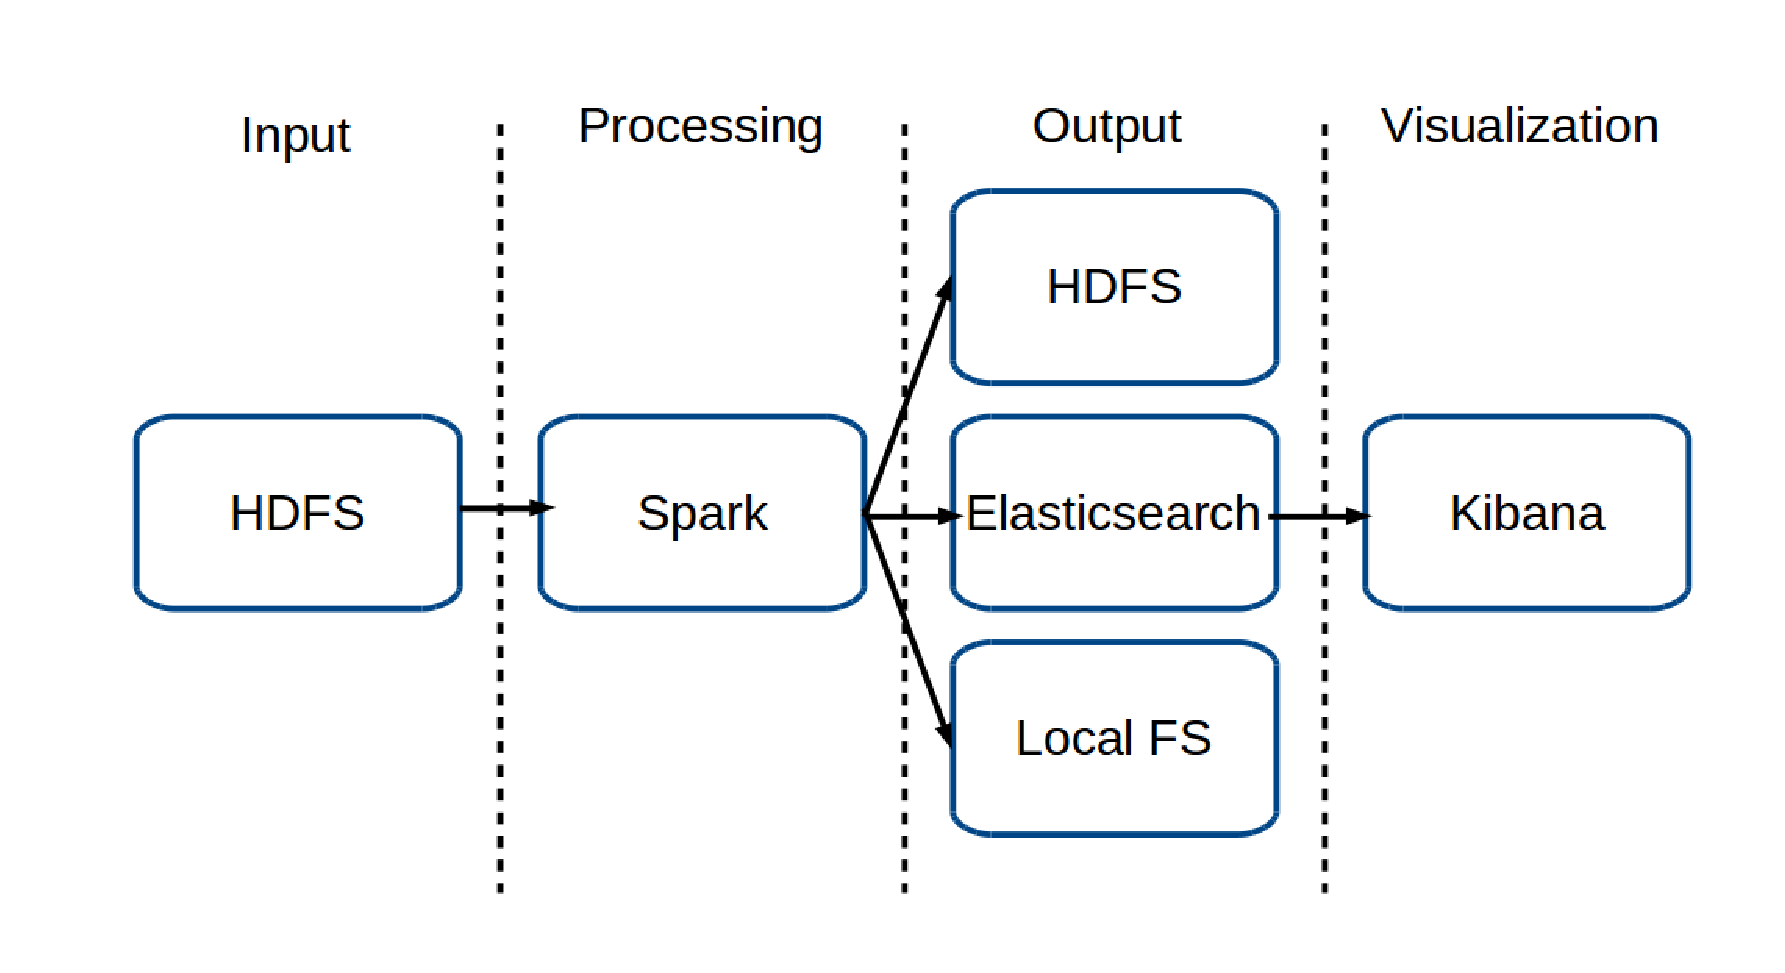
\includegraphics[width=15cm]{structure.eps}\hspace{2pc}%
\caption{\label{fig:structure}Structure of CMS dataset block replica monitoring system}
\end{center}
\end{figure}

\section{Input, processing and output}

Block replicas data snapshot has a size ranging from 2 to 3.5 gigabytes and currently expanding. Considering long term solution it was decided to keep this data and export daily snapshots in 
Hadoop file system [5]. It provides advantages of scalability, effectiviness and resilience to failure.

Block replicas snapshot contains many informative fields which cannot be analysed all at once. To fix this issue system had to provide a mean of reducing data dimensions. Dynamic aggregation 
is the core of this approach which lets reduce complexity of data for every service execution. Service allows to define one or more grouping keys, one or more result values and for each 
result value aggregation type can be specified. Aggregations include basic operations such as sum, count, min, max, first, last, mean. For better data analysis two extra operations were implemented: 
day avarage which simply sums all results fields and divides it by distinct count of days and delta operation which shows data movement between sites in customizable date periods. Approach 
also suggests data ordering and data filtering (by one or more fields) features. For text field filtering regular expressions were used. It allows to reduce non-informative amount of information to 
a minimum value. As efficieny was one of the main goals of the approach, to implement processing module Spark [6]  technology was chosen. It allowed to make a use of existing CMS network 
infrastructure and provided advantages of distributed computing and memory processing. Related to study [7]  dataframes and sparkSQL were used instead of rdds and map/reduce for performance 
improvements. All algorithms in aggregation process were implemented in manner that reduces data shuffling through the network as much as possible (shuffling large amounts of data results in performance 
issues). 

Proposed approach suggests few possibilities to store results. Every of them is supposed to be used for specific purposes.
\begin{itemize}
\item Hadoop file system. Should be used for long-term storage. 
\item Local file system. Should be used for quick aggregations stored in personal environment. Aggregation abstraction level should be chosen appropriately in order to get small files. 
This option requires data collection to master node and might fill all available memory on master node.
\item Elasticsearch resource [8]. Should be used with data that needs to be visualized. Configurability is one of the most important goals of the approach, so elasticsearch has dedicated 
configuration file with options to configure node, port and resource(index/type). Using third-party package [9] allowed to make direct connection from spark to elasticsearch resource 
without a need to have an extra step. When writing data to elasticsearch extra field "origin" is added to schema. As service can be run for different purposes (cronjob or custom execution) 
extra field helps to solve data distinction issues. It is also very important for Kibana visualization to filter proper data for dashboards.
\end{itemize}

\section{Performance}

Having good performance on data processing was one of the most important goals of this approach. Using different measures to achieve this goal allowed service to reduce processing time to a 
minimum. As different aggregations have different performance results we provide two performance figures on different aggregations (sum is considered to be low-cost operation and delta is 
considered to be computationaly expensive operation). It is worth mentioning that both aggregations was processed in yarn mode. Allocated resources (not necessarily used) are written in the 
performance tables \ref{tab:performance-sum}, \ref{tab:performance-delta}.

\begin{itemize}
\item Group keys: now, user group, acquisition era, data tier, node kind
\item Result fields: node bytes, destination bytes
\item Aggregations: sum, sum
\item Output: Hadoop file system
\end{itemize}

\begin{table}[h]
\begin{center}
\caption{Performance of basic aggregations}
\label{tab:performance-sum}
\begin{tabular}{l*{6}{c}r}
\br
Interval 	   & Input	     & Cores	      & Memory 		& Output 	  & Duration \\
\mr
1 day              & ~3GB            & 65             & 361472MB        & ~600KB          & ~1.6min \\
1 month            & ~100GB          & 65             & 361472MB        & ~18MB           & ~4.3min \\
3 months           & ~310GB          & 65             & 361472MB        & ~52MB  	  & ~9.7min \\
1 year             & ~1.1TB          & 65             & 361472MB        & ~186MB          & ~28min \\
\br
\end{tabular}
\end{center}
\end{table}
\begin{itemize}
\item Group keys: now, node name
\item Result fields: node bytes
\item Aggregations: delta
\item Interval: 1
\item Output: hadoop file system
\end{itemize}
\begin{table}[h]
\begin{center}
\caption{Performance of delta aggregations}
\label{tab:performance-delta}
\begin{tabular}{l*{6}{c}r}
\br
Interval	   & Input	     & Cores	      & Memory		& Output 	  & Duration \\
\mr
2 days             & ~5GB            & 65             & 361472MB        & ~12.7KB         & ~2.5min \\
7 days             & ~20GB           & 65             & 361472MB        & ~41.6KB         & ~4min \\
1 month            & ~90GB           & 65             & 361472MB        & ~189.2KB  	  & ~8.5min \\
6 months           & ~500GB          & 65             & 361472MB        & ~1MB            & ~35min \\
\br
\end{tabular}
\end{center}
\end{table}

\section{Visualization}

Structure of analysis service allows to reduce the complexity of visualization process to a minimal level. Having data in elasticsearch resource lets to use visualization technologies 
built on top of it. In this approach Kibana [10] was used. From programmatic perspective Kibana configuration is the only process that needs to be done. Analytic himself then can 
make searches, visualizations and compose dashboards to fulfil his own needs. One of the example usage of kibana can be seen in figure \ref{fig:pie-charts}. It simply shows two user groups 
(analysisops, dataops) storage distribution of top 10 storage consuming acquisition eras.

\begin{figure}[h]
\begin{center}
\includegraphics[width=15cm]{pie-charts.eps}\hspace{2pc}%
\caption{\label{fig:pie-charts}Kibana visualization of block replicas data (current)}
\end{center}
\end{figure}

Another example in figure \ref{fig:bar-charts} shows data distribution of top 10 storage consuming data tiers. It is visualized in time perspective. 

\begin{figure}[h]
\begin{center}
\includegraphics[width=15cm, height=7cm]{bar-charts.eps}\hspace{2pc}%
\caption{\label{fig:bar-charts}Kibana visualization of block replicas data (historical)}
\end{center}
\end{figure}

\section{Conclusions}

Proposed approach helps to analyze data by reducing its dimensions (aggregation) and visualizing it. It has three main advantages. First of all, it is very 
efficient as it is build on top of Spark which allows distributed computing using executors memory instead of disk. Also, it is fully-covered. This approach provides a possibility to
get everything from raw data in hadoop file system to visualizations and dashboards in Kibana. Lastly, it is highly configurable. If there is a need to look at 
data from different perspective only service parameters must be changed. This results in different agregations, different results written in Hadoop file system and Elasticsearch, 
different visualizations and dashborads in Kibana. All of this without a need to change the service itself.

\section*{References}
\medskip
\begin{thebibliography}{9}
\item The CMS collaboration 2008 The CMS experiment at the CERN LHC {\it JINST} {\bf 3} S08004
\item Eck C {\it et al.} 2005 LHC Computing Grid Technical Design Report {\it CERN-LHCC-2005-024}
\item Egeland R, Metson S and Wildish T 2008 Data transfer infrastructure for CMS data taking. {\it XII Advanced Computing and Analysis Techniques in Physics Research (Erice, Italy: 
Proceedings of Science)}
\item Giffels M, Guo Y, Kuznetsov V, Magini N and Wildish T 2014 The CMS Data Management System {\it J. Phys.: Conf. Ser.} {\bf 513} 042052 
\item http://hadoop.apache.org/ 
\item http://spark.apache.org/
\item https://databricks.com/blog/2015/02/17/introducing-dataframes-in-spark-for-large-scale-data-science.html
\item https://www.elastic.co/products/elasticsearch
\item https://www.elastic.co/products/hadoop 
\item https://www.elastic.co/products/kibana
\end{thebibliography}
\smallskip

\end{document}


